% Created 2022-06-30 Thu 15:25
% Intended LaTeX compiler: pdflatex
\documentclass[presentation]{beamer}
\usepackage{relsize}
\usepackage[utf8]{inputenc}
\usepackage[T1]{fontenc}
\usepackage{graphicx}
\usepackage{longtable}
\usepackage{wrapfig}
\usepackage{rotating}
\usepackage[normalem]{ulem}
\usepackage{amsmath}
\usepackage{amssymb}
\usepackage{capt-of}
\usepackage{hyperref}
\mode<beamer>{\usetheme{Madrid}}
\usepackage[super]{natbib}
\usepackage{url}
\makeatletter
\setbeamertemplate{footline}{
\leavevmode%
\hbox{%
\begin{beamercolorbox}[wd=.2\paperwidth,ht=2.25ex,dp=1ex,center]{author in head/foot}%
\usebeamerfont{author in head/foot}\insertshortauthor\expandafter\ifblank\expandafter{\beamer@shortinstitute}{}{~~(\insertshortinstitute)}
\end{beamercolorbox}%
\begin{beamercolorbox}[wd=.57\paperwidth,ht=2.25ex,dp=1ex,center]{title in head/foot}%
\usebeamerfont{title in head/foot}\insertshorttitle
\end{beamercolorbox}%
\begin{beamercolorbox}[wd=.23\paperwidth,ht=2.25ex,dp=1ex,right]{date in head/foot}%
\usebeamerfont{date in head/foot}\insertshortdate{}\hspace*{2em}
\insertframenumber{} / \inserttotalframenumber\hspace*{2ex}
\end{beamercolorbox}}%
\vskip0pt%
}
\makeatother
\author[Marco A. Gallo]{Marco A. Gallo\\ \vspace{1mm}Supervisor: Dr. Matthia Sabatelli}
\institute[]{University of Groningen}
\setbeamertemplate{itemize items}[default]
\setbeamertemplate{enumerate items}[default]
\setbeamertemplate{caption}[numbered]
\setbeamertemplate{navigation symbols}{}
\usetheme{default}
\date{29-06-2022}
\title{Using Ensembles to address Bootstrapping Error in Offline RL}
\hypersetup{
 pdfauthor={},
 pdftitle={Using Ensembles to address Bootstrapping Error in Offline RL},
 pdfkeywords={},
 pdfsubject={},
 pdfcreator={Emacs 28.1 (Org mode 9.5.2)},
 pdflang={English}}
\begin{document}

\maketitle
\begin{frame}{Outline}
\tableofcontents
\end{frame}


\section{Background}
\label{sec:org8eff8cd}
\begin{frame}[label={sec:orgb976866}]{Reinforcement Learning - A schematic view}
\begin{figure}[htbp]
\centering
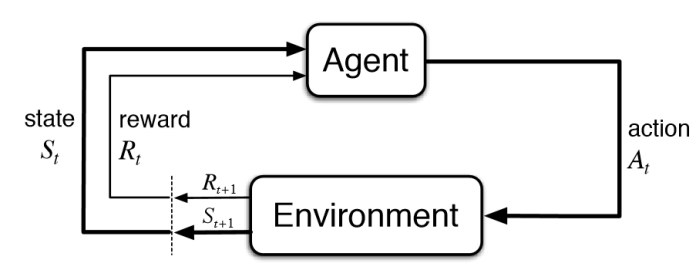
\includegraphics[width=\textwidth]{./online_rl_loop.jpg}
\caption{\label{fig:org5d2cec5}The agent-environment loop (\citeauthor{sutton2018reinforcement}, \citeyear{sutton2018reinforcement})}
\end{figure}
\end{frame}

\begin{frame}[label={sec:org2be580b}]{Reinforcement Learning Problem Statement}
\begin{itemize}
\item An agent seeking an optimal policy \(\pi(s, a)\) - a mapping from
states to action probabilities (\(s \in \mathcal{S}\), \(a \in \mathcal{A}\))
\item Used in sequential decision making problems modeled as Markov
decision process (\emph{MDP}), enriched with a reward function \(R(s, a)
  \colon \mathcal{S} \times \mathcal{A} \mapsto \mathbb{R}\)
\end{itemize}

\begin{itemize}
\item Focus: \emph{value-based}, \emph{model-free} methods
\end{itemize}
\end{frame}

\begin{frame}[label={sec:orgf63bec7}]{Reinforcement Learning (RL) - Offline}
\begin{figure}[htbp]
\centering
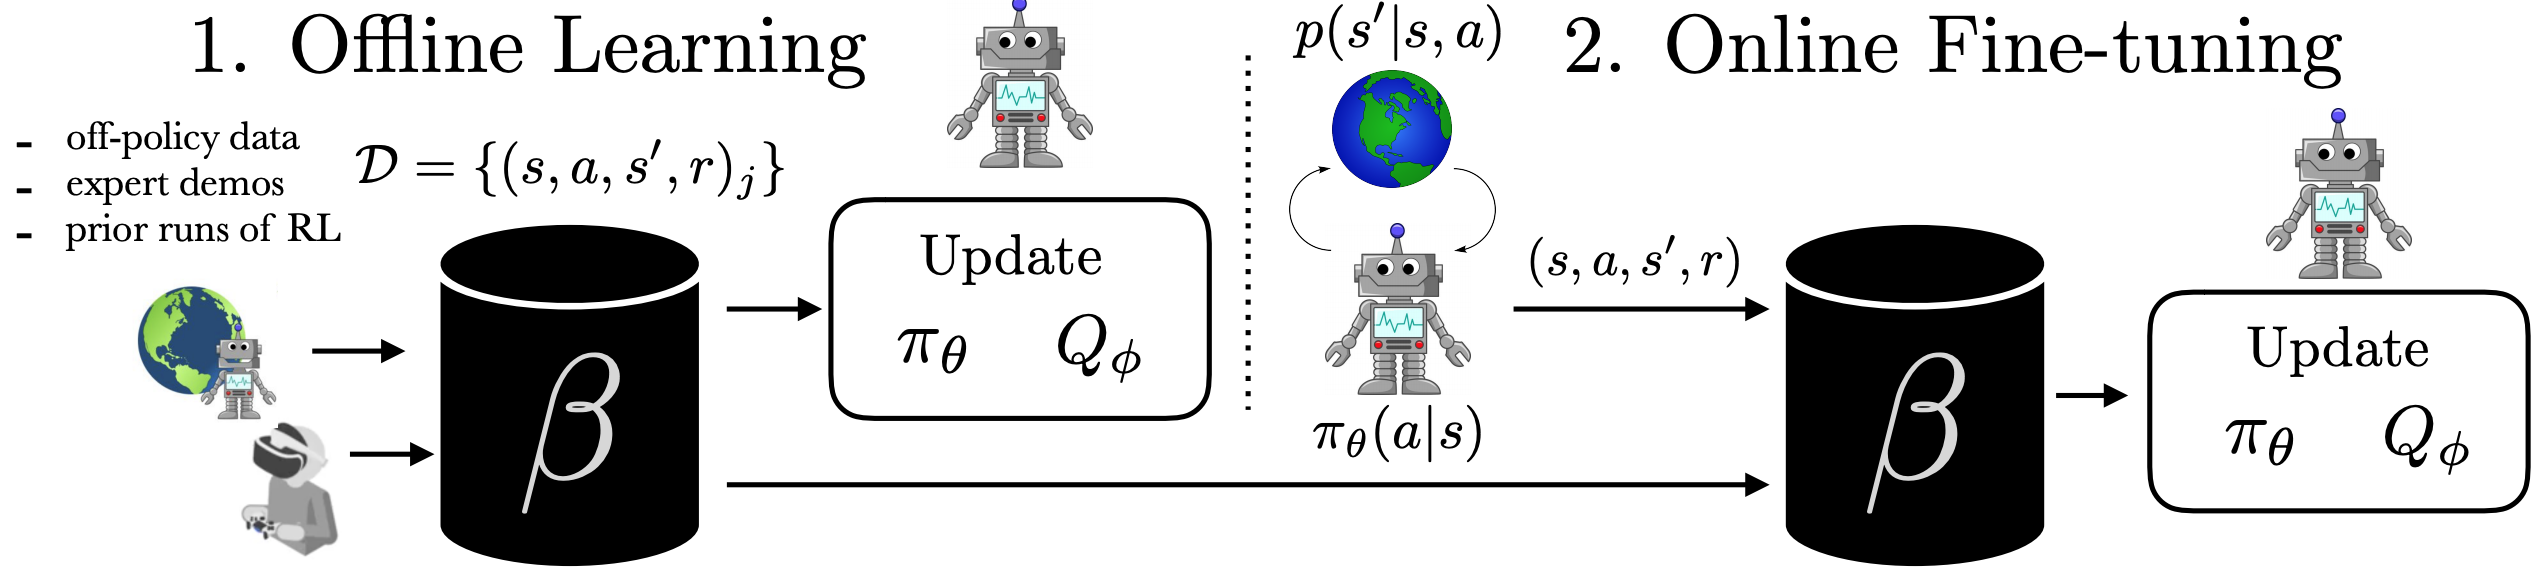
\includegraphics[width=\textwidth]{./offline_rl_sketch_2.png}
\caption{\label{fig:org2dc03a4}The learning loop in Offline RL, courtesy of \citeauthor{DBLP:journals/corr/abs-2006-09359}}
\end{figure}

\begin{itemize}
\item Also called Batch Reinforcement Learning
\item Behavior policy \(\pi_{\beta}\) generates dataset \(\mathcal{D}\)
\item \emph{Pure Batch} vs \emph{Growing Batch} methods
\end{itemize}
\end{frame}

\section{Offline RL is hard}
\label{sec:orgd12c9fa}
\begin{frame}[label={sec:org59048a2}]{Detrimental factors in Offline RL}
\begin{itemize}
\item Function approximation errors in Deep RL (Neural Networks)
\end{itemize}

\begin{itemize}
\item Different state visitation frequencies under training and testing
distributions
\end{itemize}

\begin{itemize}
\item \alert{Bootstrapping error} (\citeauthor{kumar2019stabilizing},
\citeyear{kumar2019stabilizing})
\end{itemize}
\end{frame}

\begin{frame}[label={sec:org537c921}]{Bootstrapping Error}
DQN objective function:
\begin{equation*}
\mathcal{L}(\theta) = \mathbb{E}_{\langle s_t, a_t, r_t, s_{t+1} \rangle \sim D}\left[(r_t + \gamma \max_{a\in\mathcal{A}}Q(s_{t+1,a;\theta^{-}}) - Q(s_t, a_t;\theta))^2\right]
\end{equation*}

\begin{figure}[htbp]
\centering
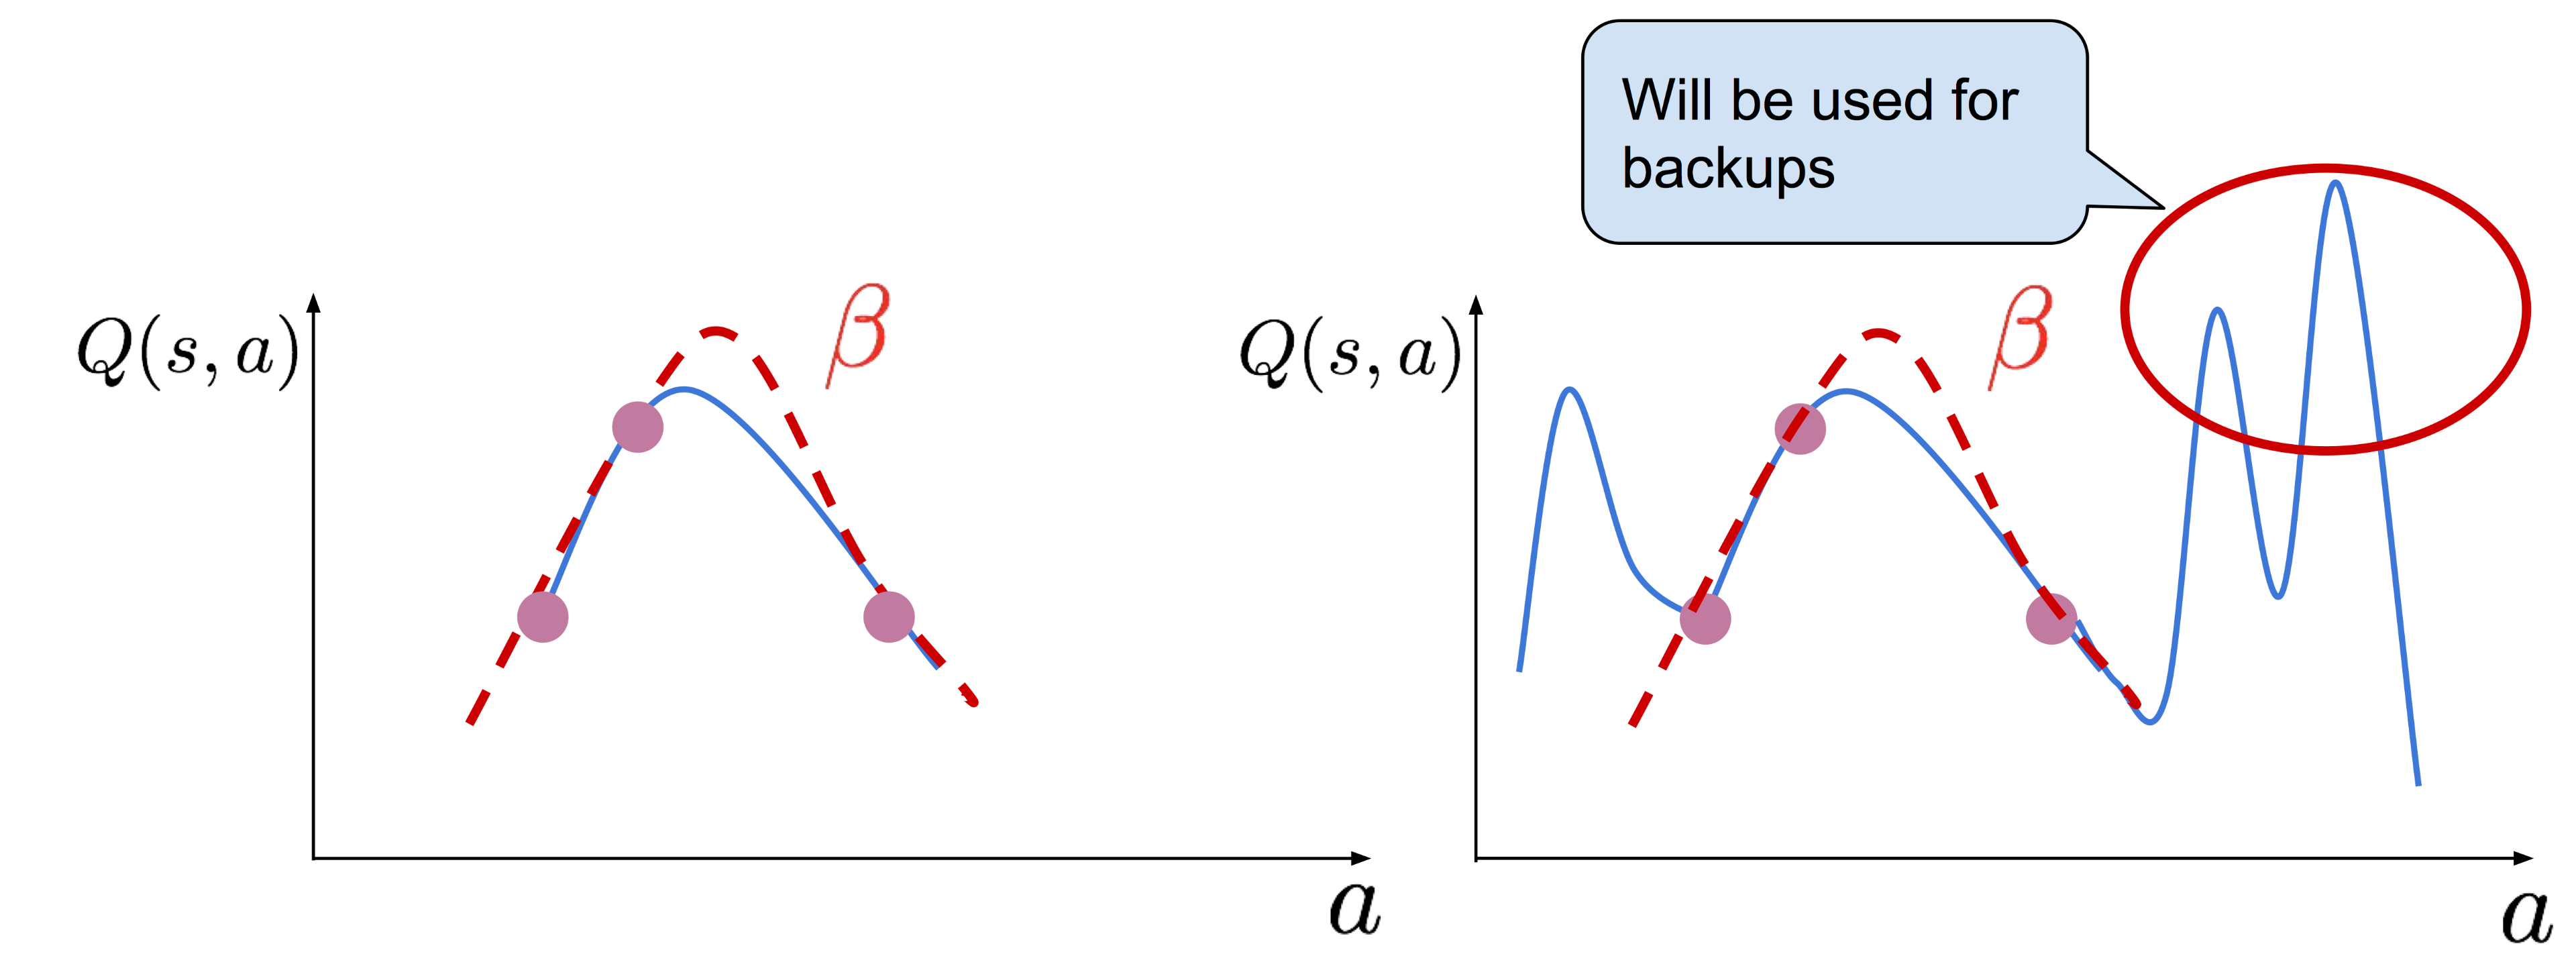
\includegraphics[width=.9\linewidth]{./bootstrap_error_offline_rl.png}
\caption{\label{fig:org7890d7a}Incorrectly high Q-values for OOD actions may be used for backups, leading to accumulation of error. Figure and caption: \citeauthor{kumar}}
\end{figure}
\end{frame}

\begin{frame}[label={sec:org8d94f9a}]{Bootstrapping Error in the DQV\cite{sabatelli2020deep} algorithmic family}
\begin{itemize}
\item We want to check if the DQV and DQV-Max deep RL algorithms suffer
from the Bootstrapping Error in the \emph{offline} setting
\item DQV objective functions:
\fontsize{9pt}{10pt}\selectfont
\begin{align}
\mathcal{L}(\phi) &= \mathbb{E}_{\langle s_t, a_t, r_t, s_{t+1} \rangle \sim D}\left[(r_t + \gamma V(s_{t+1};\phi^{-}) - V(s_t;\phi))^2\right] \\
\mathcal{L}(\theta) &= \mathbb{E}_{\langle s_t, a_t, r_t, s_{t+1} \rangle \sim D}\left[(r_t + \gamma V(s_{t+1};\phi^{-}) - Q(s_t;\theta))^2\right]
\end{align}
\item DQV-Max objective functions:
\fontsize{9pt}{10pt}\selectfont
\begin{align}
\label{eq:org2ddb2f3}
\mathcal{L}(\phi) &= \mathbb{E}_{\langle s_t, a_t, r_t, s_{t+1} \rangle \sim D}\left[(r_t + \gamma \max_{a\in\mathcal{A}}Q(s_{t+1},a;\theta^{-}) - V(s_t;\phi))^2\right] \\
\mathcal{L}(\theta) &= \mathbb{E}_{\langle s_t, a_t, r_t, s_{t+1} \rangle \sim D}\left[(r_t + \gamma V(s_{t+1};\phi) - Q(s_t, a_t;\theta))^2\right]
\end{align}
\end{itemize}
\end{frame}

\begin{frame}[label={sec:org40d31b9},fragile]{Experimental setup}
 \begin{itemize}
\item Classic control OpenAI Gym environments: \texttt{CartPole-v1} and
\texttt{Acrobot-v1}
\item Data collection: log every trajectory \(\langle
  s,a,r,s^{\prime}\rangle\) of a DQN\cite{mnih2013playing} agent
trained online for 500k steps
\item Hyper-parameters and training scheme follow those of the
Dopamine\cite{castro18dopamine} framework
\item Record estimates of \(\max_{a \in \mathcal{A}}Q(s_{t_{0}}, a)\) at each
evaluation round to track the value estimates evolution, then compare
against ground truth
$$G_{t_{0}} = \sum_{k=0}^{T}{\gamma^{k}r_{t+k}}$$
\(T\) is the environment's finite time horizon, and \(r_{t}\)
is constant across environments
\end{itemize}
\end{frame}

\begin{frame}[label={sec:org5f884f4}]{Bootstrapping Error in the DQV algorithmic family - Results}
\begin{center}
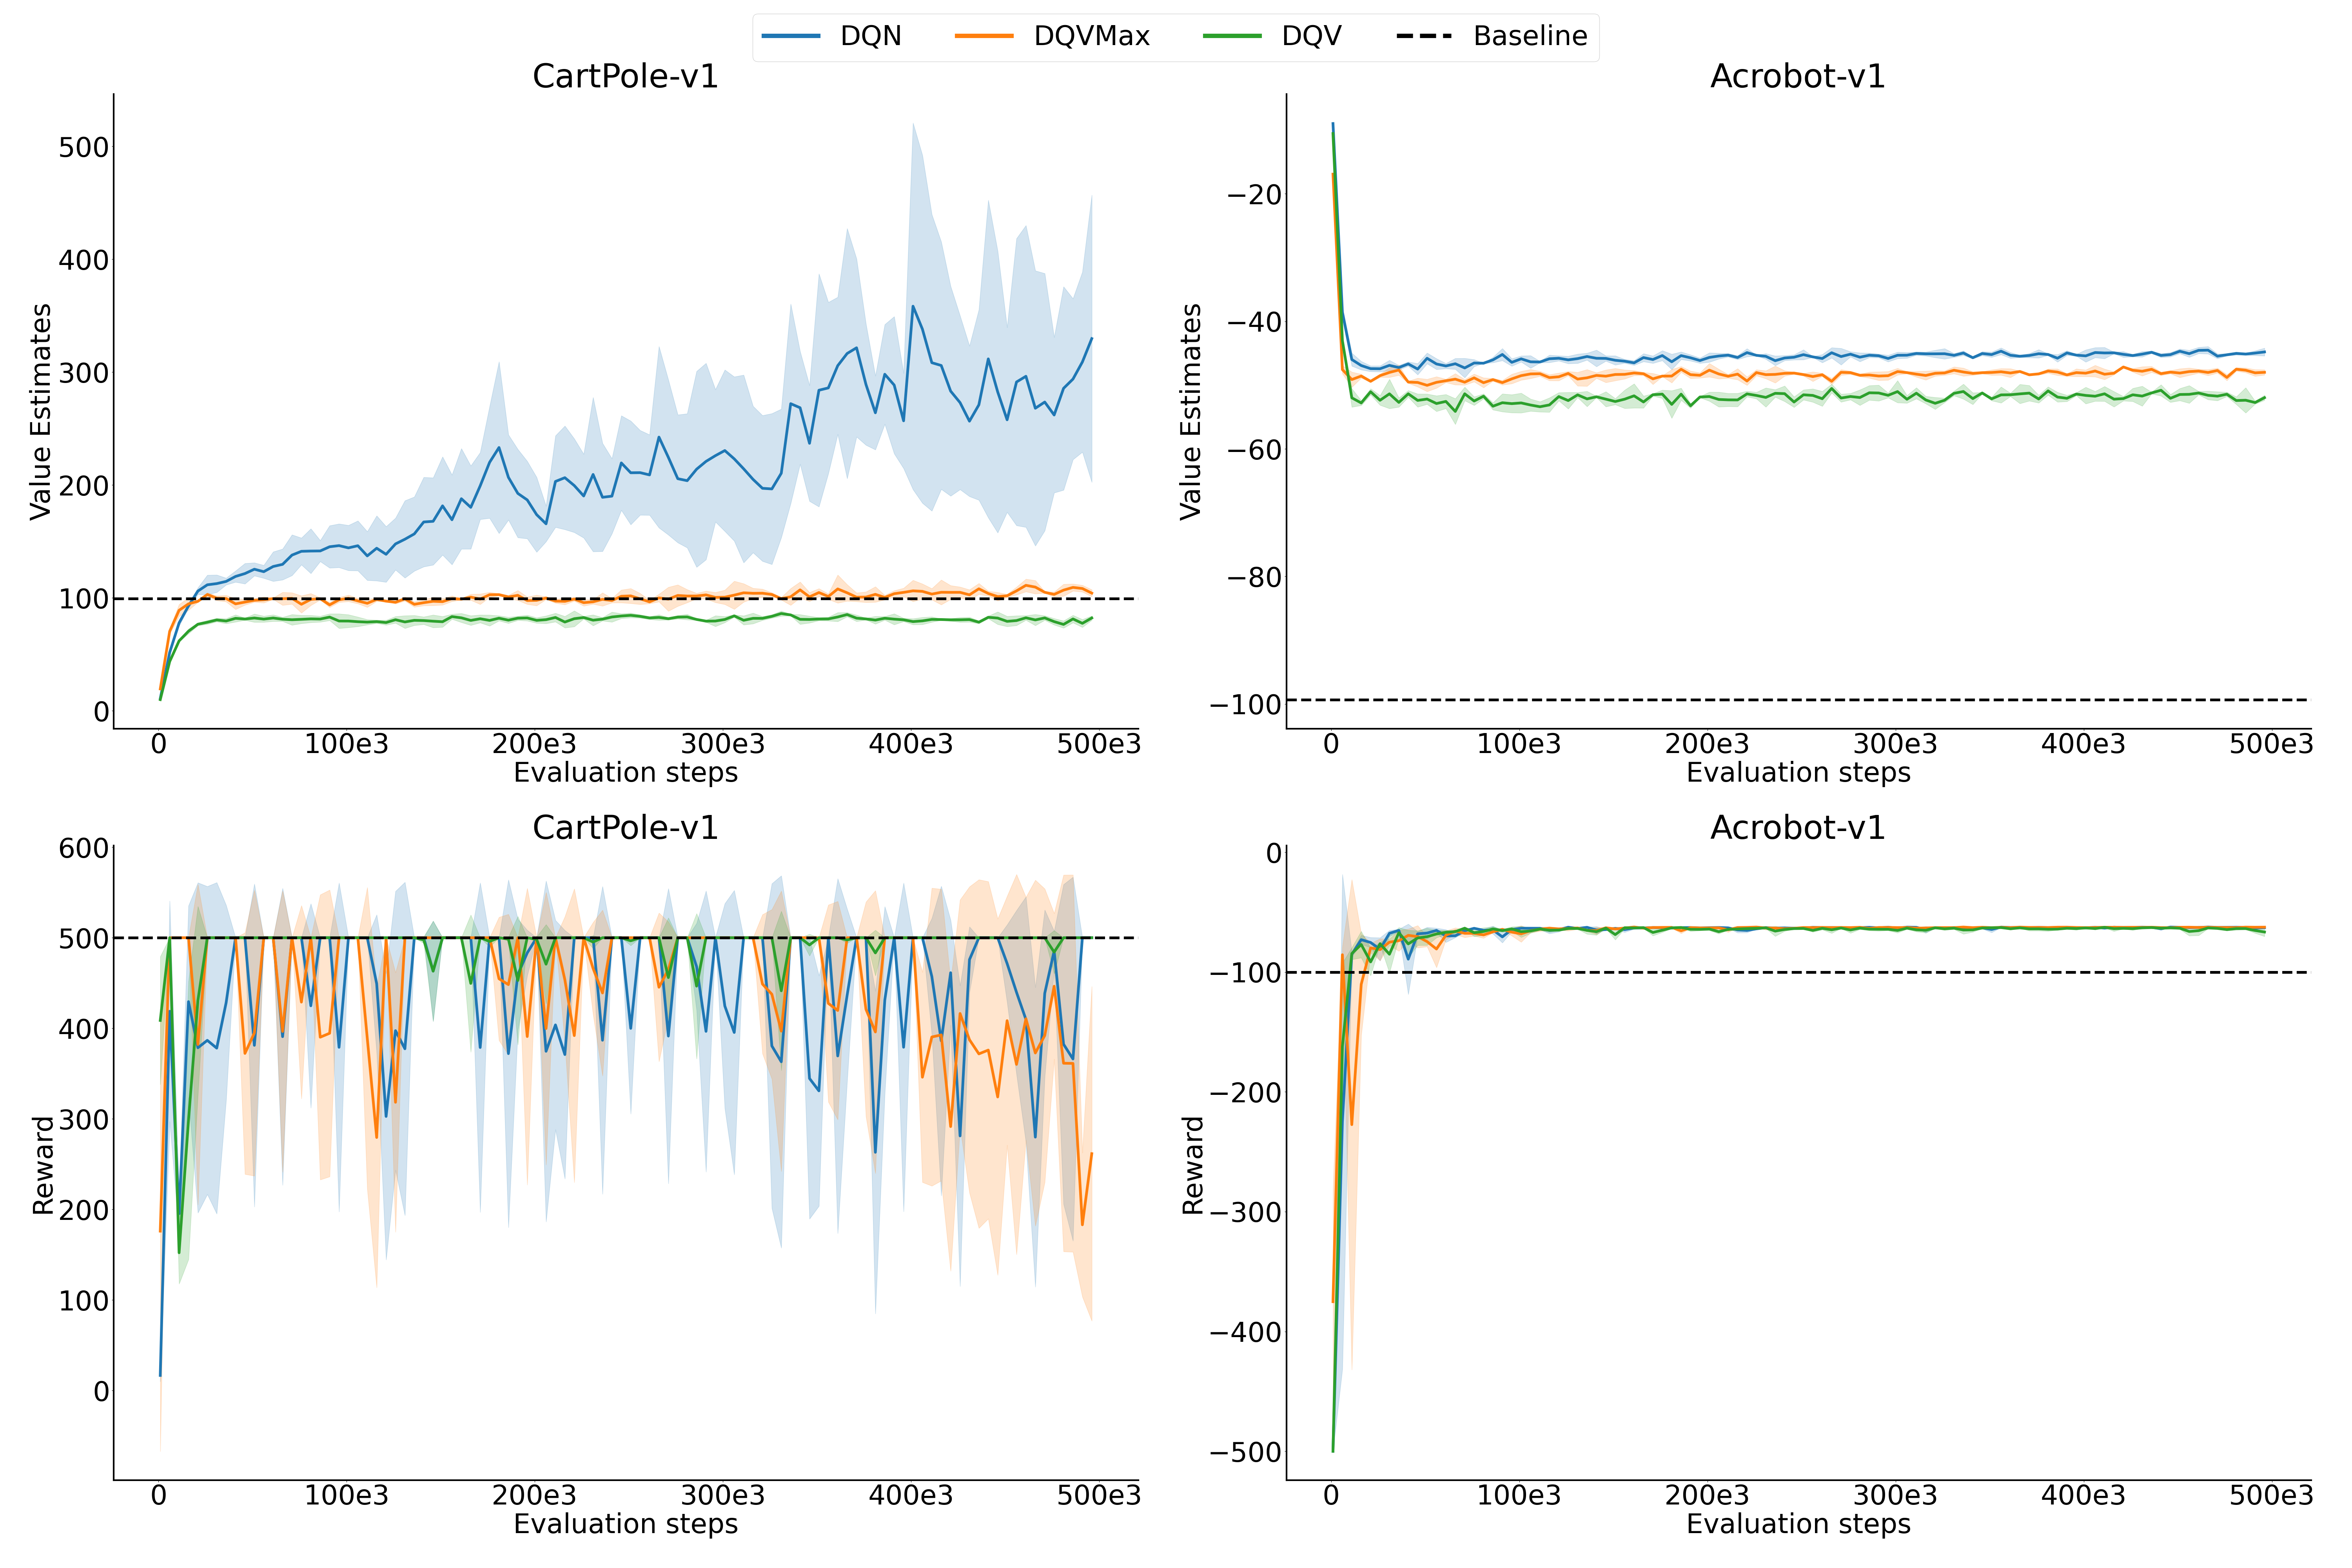
\includegraphics[width=\textwidth]{./dshift_plots_normal.png}
\end{center}
\end{frame}

\begin{frame}[label={sec:orgb925272}]{Preventing the Bootstrapping Error - Online}
Two ways of addressing the Bootstrapping Error:
\vspace{1mm}
\begin{enumerate}
\item Obtain unbiased Q-values by decoupling \emph{selection} and
\emph{evaluation}, e.g.
\begin{itemize}
\item \textbf{Double Q-Learning target}\cite{van2016deep} \\
\vspace{1mm}
\(Q^{*}\left(s, a\right) = r +\gamma Q\left(s^{\prime},
     \operatorname{argmax}_{a \in \mathcal{A}} Q^{\prime}\left(s', a \right)\right)\)
\vspace{1mm}
\item \textbf{DQV-Max targets} in Eq.(\ref{eq:org2ddb2f3}) \\

\vspace{1mm}
\end{itemize}
\item Reducing the variance of the Target Approximation Error (TAE)\cite{anschel2017averaged}
\vspace{1mm}
\begin{itemize}
\item TAE: \(Z_{s, a} = Q(s, a) - \mathbb{E}[r + \gamma \max_{a \in \mathcal{A}} Q(s', a) \vert s, a]\)
\vspace{1mm}
\item \citeauthor{anschel2017averaged} show that the magnitude of the
bootstrapping bias in Q-learning is related to the \emph{variance} of
the TAE
\end{itemize}
\end{enumerate}
\end{frame}

\begin{frame}[label={sec:org9861c8b}]{Preventing the Bootstrapping Error - Offline}
\begin{itemize}
\item In the offline setting, algorithms such as BCQ\cite{fujimoto2019off}
and BEAR\cite{kumar2019stabilizing} mitigate the Bootstrapping Error
by \emph{regularizing} the learned policy to be \emph{close} to the \emph{training
trajectories}
\item One exception: Random Ensemble Mixture
(REM)\cite{agarwal2020optimistic}
\begin{itemize}
\item Dataset \alert{size} and \alert{diversity} are crucial for offline
performance: \href{https://research.google/tools/datasets/dqn-replay/}{DQN Replay Dataset} on the Atari 2600 benchmark
\item REM idea: combining multiple noisy Q-functions creates a more
robust Q-function
\end{itemize}
\end{itemize}
\end{frame}

\section{Possible solution: Ensembles}
\label{sec:orgf6efc56}
\begin{frame}[label={sec:org2bfc36e}]{Focus: Offline DQV and DQV-Max}
DQV and DQV-Max still incur in the Bootstrapping Error, but\ldots{}
\begin{itemize}
\item Being an \emph{on-policy} algorithm, DQV is less prone to it
\item DQV-Max is \emph{off-policy}, yet it uses multiple estimators to compute
the expected Q-values \(\rightarrow\) also more robust to the
Bootstrapping Error
\item \alert{Idea}: can we use techniques for TAE reduction to improve resilience
to the Bootstrapping Error in the DQV algorithmic family?
\item Ensemble DQN\cite{anschel2017averaged}: training \(K\) Q-functions in
parallel to obtain a \(\frac{1}{K}\) variance reduction in Q-values
\item Also motivated by REM's strong offline performance
\end{itemize}
\end{frame}
\begin{frame}[label={sec:org692df91}]{Ensemble learning problem}
\fontsize{9pt}{10pt}\selectfont
\begin{itemize}
\item Ensemble DQN learning goal:
\begin{align}
\mathcal{L}(\theta) &= \frac{1}{K}\sum_{k=0}^{k-1}\mathbb{E}_{\langle s_t, a_t, r_t, s_{t+1} \rangle \sim D}\left[(r_t + \gamma \max_{a\in\mathcal{A}}Q(s_{t+1},a;\theta_{k}^{-}) - Q(s_t, a_t;\theta_{k}))^2\right]
\end{align}
\item The learning goal for DQV becomes:
\begin{align}
\mathcal{L}(\phi) &= \frac{1}{K}\sum_{k=0}^{k-1}\mathbb{E}_{\langle s_t, a_t, r_t, s_{t+1} \rangle \sim D}\left[(r_t + \gamma V(s_{t+1};\phi_{k}^{-}) - V(s_t;\phi_{k}))^2\right] \\
\mathcal{L}(\theta) &= \frac{1}{K}\sum_{k=0}^{k-1}\mathbb{E}_{\langle s_t, a_t, r_t, s_{t+1} \rangle \sim D}\left[(r_t + \gamma V(s_{t+1};\phi_{k}^{-}) - Q(s_t, a_t;\theta))^2\right]
\end{align}
\item The learning goal for DQV-Max becomes:
\begin{align}
\label{eq:org093b6f2}
\mathcal{L}(\phi) &= \frac{1}{K}\sum_{k=0}^{k-1}\mathbb{E}_{\langle s_t, a_t, r_t, s_{t+1} \rangle \sim D}\left[(r_t + \gamma \max_{a\in\mathcal{A}}Q(s_{t+1},a;\theta_{k}^{-}) - V(s_t;\phi_{k}))^2\right] \\
\mathcal{L}(\theta) &= \frac{1}{K}\sum_{k=0}^{k-1}\mathbb{E}_{\langle s_t, a_t, r_t, s_{t+1} \rangle \sim D}\left[(r_t + \gamma V(s_{t+1};\phi_{k}) - Q(s_t, a_t;\theta_{k}))^2\right]
\end{align}
\end{itemize}
\end{frame}
\section{Results}
\label{sec:orgbe4cfb5}
\begin{frame}[label={sec:org235f3e6}]{Ensemble Architecture}
\begin{figure}[htbp]
\centering
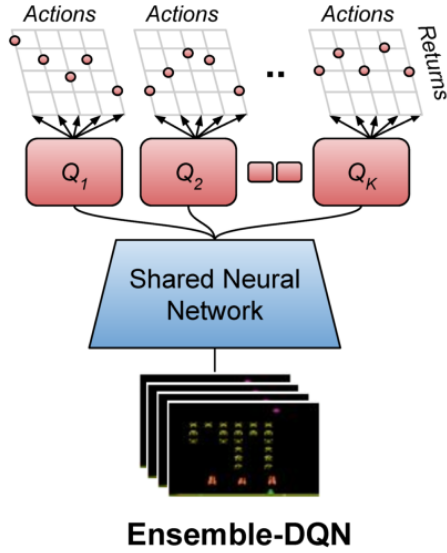
\includegraphics[width=.45\textwidth]{./hydra_nn_arch.png}
\caption{\label{fig:orgd7aec56}Multi-head Neural Network from \citeauthor{agarwal2020optimistic}}
\end{figure}
\end{frame}

\begin{frame}[label={sec:org2735942}]{Bootstrapping Error with Multi-Headed DQV agents}
\begin{center}
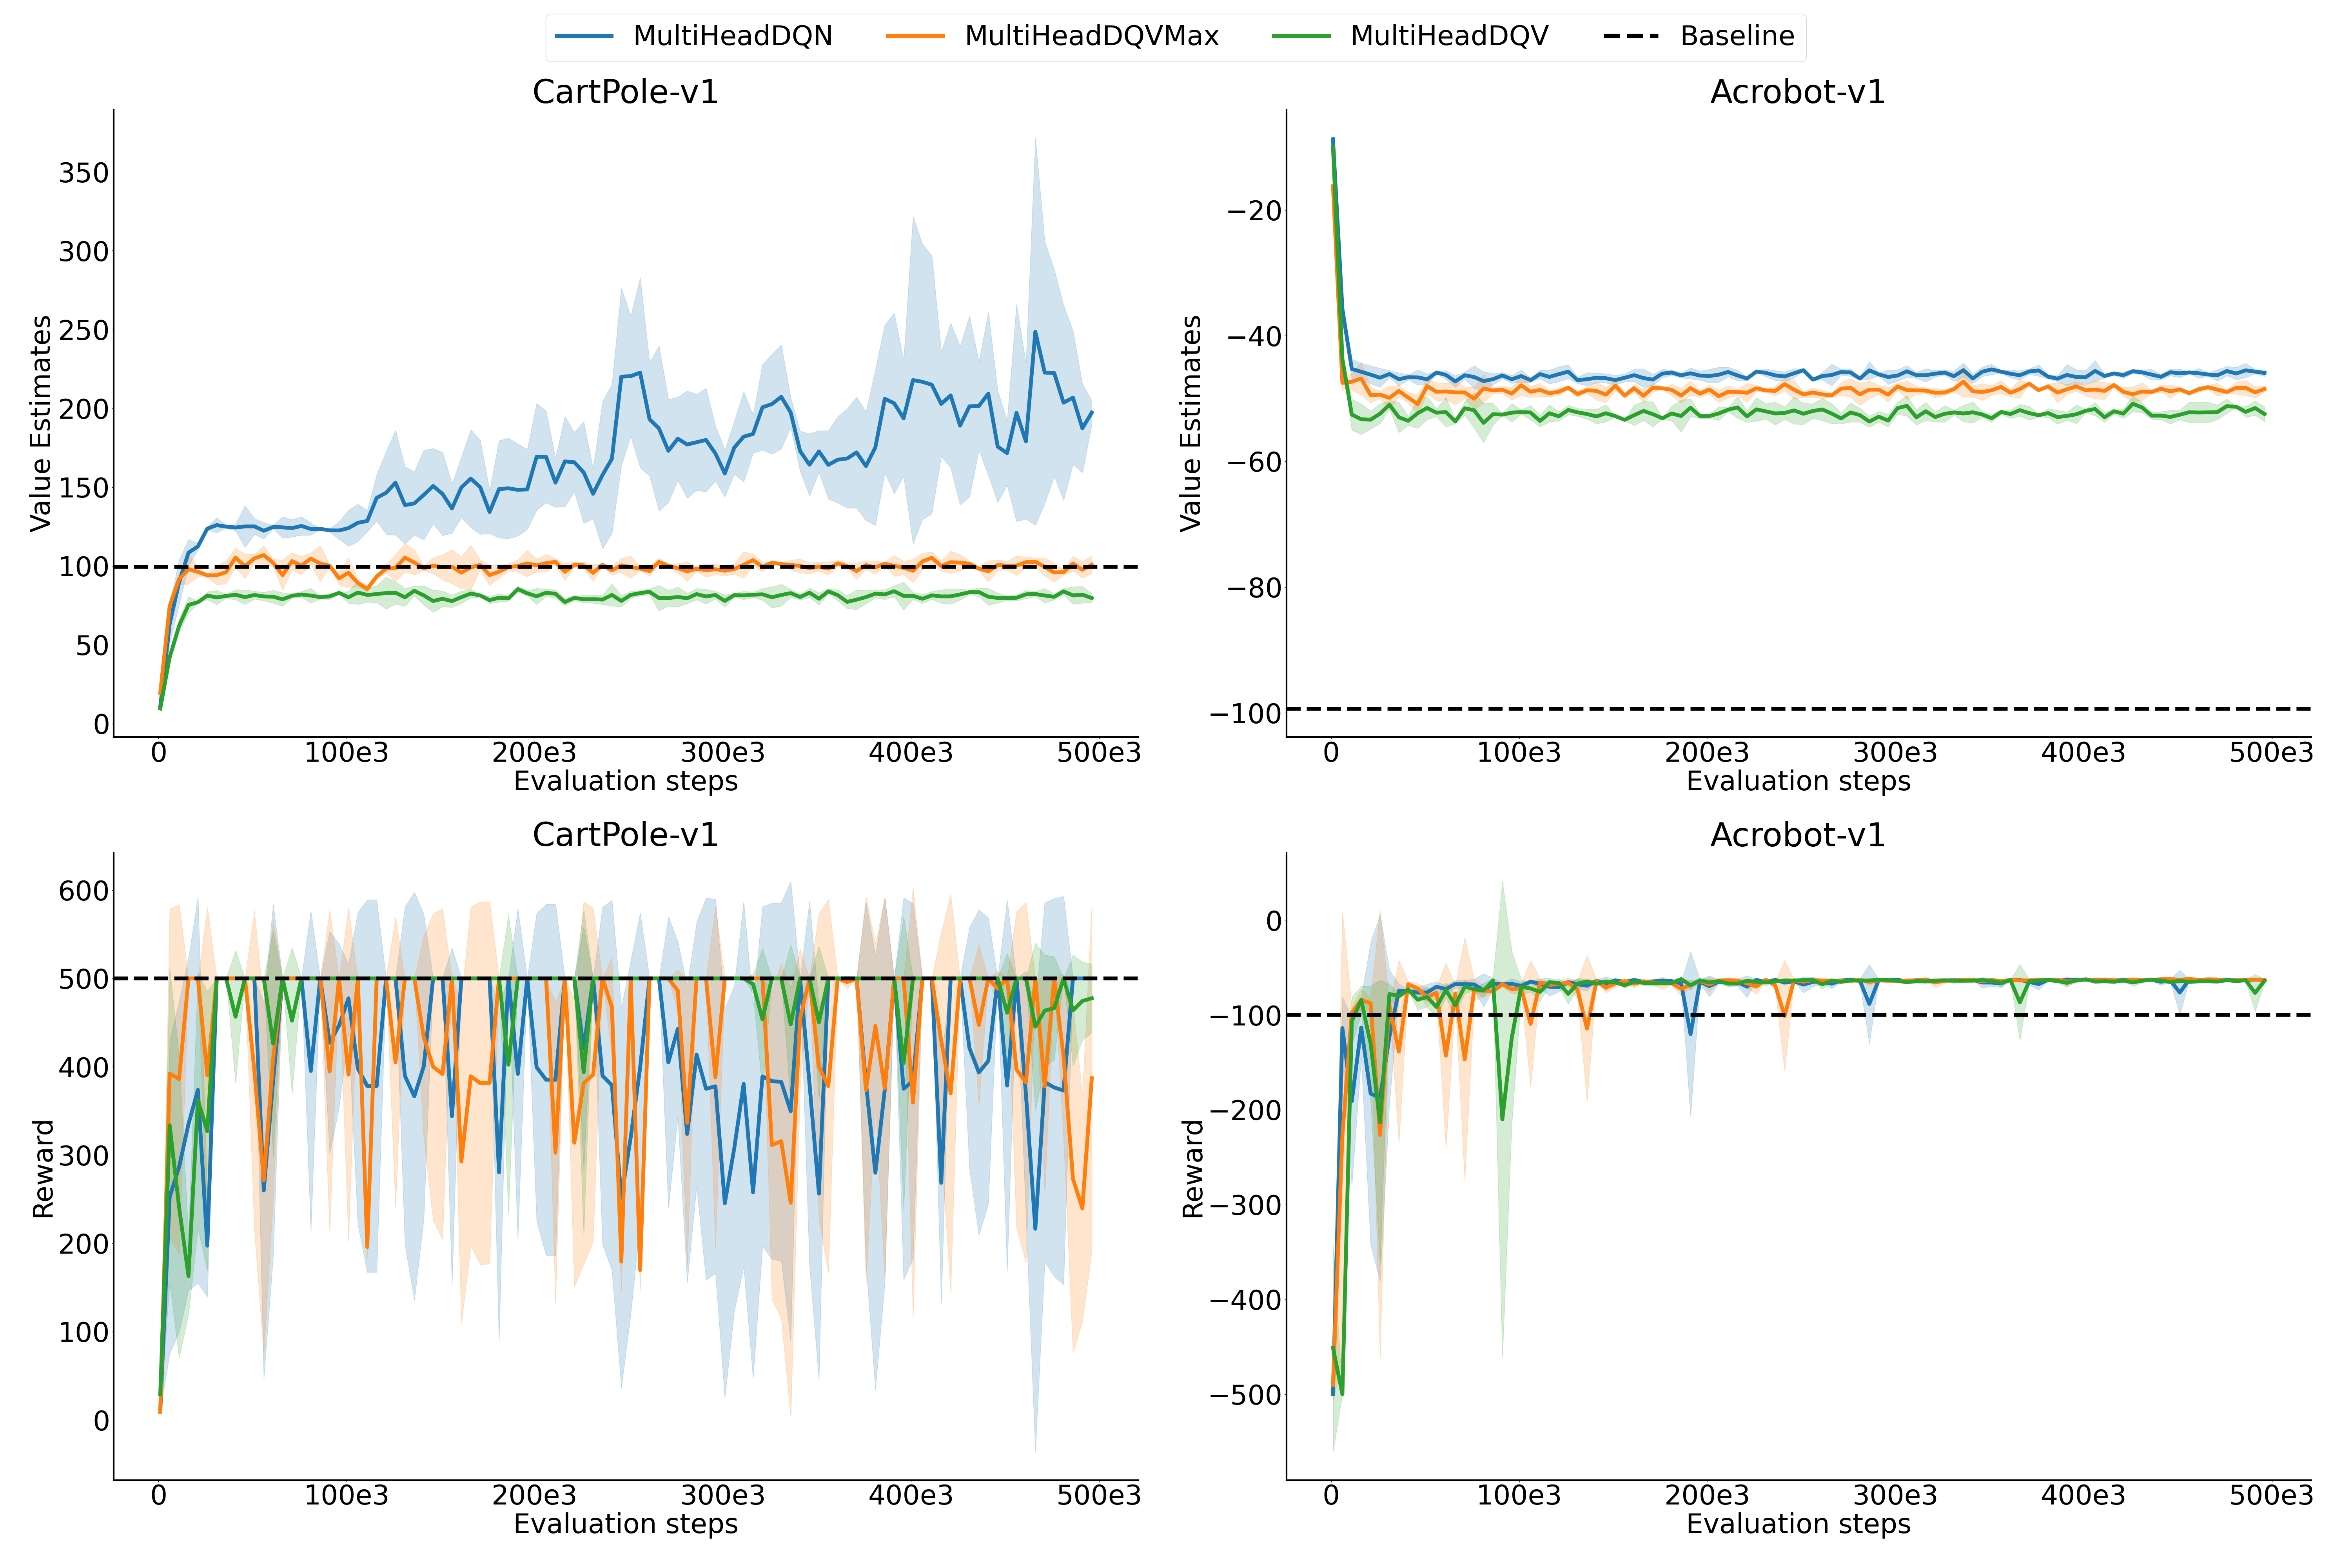
\includegraphics[width=\textwidth]{./dshift_plots_ensembles.png}
\end{center}
\end{frame}

\section{Analysis}
\label{sec:orgba7a492}
\begin{frame}[label={sec:org4c114e6}]{Conclusions}
\begin{itemize}
\item No real improvement over the traditional DQV algorithms
\item The decoupling of estimation and update in the off-policy DQV-Max
is stronger than the gains from multiple estimation observed with
base DQN
\item Rigorous analysis of the TAE for the DQV algorithms needed
\end{itemize}
\end{frame}
\section{References}
\label{sec:org755a433}
\begin{frame}[allowframebreaks]{References}
\bibliographystyle{apalike}
\bibliography{bibliography}
\end{frame}
\end{document}